\documentclass[12pt, letterpaper]{article}

\usepackage[utf8]{inputenc}
\usepackage[T1]{fontenc}
\usepackage[spanish]{babel}
\usepackage{geometry}
\usepackage{graphicx}
\usepackage{float}
\usepackage{booktabs}
\usepackage{longtable}
\usepackage{array}
\usepackage{amsmath}
\usepackage{amssymb}
\usepackage{xcolor}
\usepackage{caption}
\usepackage{subcaption}
\usepackage{fancyhdr}
\usepackage{hyperref}
\usepackage{enumitem}
\usepackage{tocbibind}

\geometry{
    top=2.5cm,
    bottom=2.5cm,
    left=2.5cm,
    right=2.5cm
}

\hypersetup{
    colorlinks=true,
    linkcolor=black,
    urlcolor=blue,
    citecolor=black
}

\setlength{\parskip}{6pt}
\setlength{\parindent}{0pt}

\pagestyle{fancy}
\fancyhf{}
\fancyhead[L]{CE1111 -- Análisis Numérico}
\fancyhead[R]{Enfriamiento de una barra}
\fancyfoot[C]{\thepage}
\setlength{\headheight}{15pt}

% -------------------------
% DATOS DEL INFORME
% -------------------------
\newcommand{\universidad}{Instituto Tecnológico de Costa Rica}
\newcommand{\curso}{CE1111 -- Análisis Numérico para Ingeniería}
\newcommand{\titulo}{Aplicación -- Enfriamiento de una barra}
\newcommand{\estudiantes}{%
    Joaquin Ignacio Ramirez Sequeira\\
    Joseph Stif Piedra Montero%
}
\newcommand{\profesor}{Juan Pablo Soto Quirós}
\newcommand{\semestre}{Semestre II, 2026}
\newcommand{\fecha}{\today}

\begin{document}


\begin{titlepage}
    \centering
    \vspace*{1cm}
    {\Large\textbf{\universidad}\par}
    \vspace{1.5cm}
    % \includegraphics[width=0.22\textwidth]{logo.png}
    \vspace{1cm}
    {\large\curso\par}
    \vspace{2cm}
    {\LARGE\bfseries \titulo\par}
    \vspace{0.8cm}
    {\large Informe de resultados\par}
    \vspace{2cm}
    \begin{flushleft}
        \textbf{Estudiantes:}\\
        \estudiantes
        \vspace{0.6cm}

        \textbf{Docente:}\\
        \profesor
        \vspace{0.6cm}

        \textbf{Periodo académico:}\\
        \semestre
    \end{flushleft}
    \vfill
    {\large \fecha\par}
\end{titlepage}


\tableofcontents
\newpage

% =================================================
\section{Introducción}
% =================================================

En este informe se presentan los resultados obtenidos al resolver la ecuación de calor unidimensional aplicada al enfriamiento de una barra metálica. El problema consiste en aproximar la evolución de la temperatura en una barra de longitud \(L=1\) m, con difusividad térmica \(\alpha=0.01\) m\(^2\)/s, extremos mantenidos a \(20^\circ\)C y una condición inicial dada por \(T(x,0)=20+80\sin(\pi x/L)\).

Para ello se utilizaron tres esquemas de diferencias finitas: Euler explícito, Euler implícito y Crank--Nicolson. Los esquemas implícitos se resolvieron mediante el método de Gradiente Conjugado, implementado previamente en la Parte 1 del bloque. El objetivo principal es comparar los esquemas en términos de precisión, costo computacional y estabilidad, y determinar el instante en que toda la barra alcanza una temperatura menor o igual a \(30^\circ\)C.

% =================================================
\section{Deducción de los esquemas}
% =================================================

\subsection{Cambio de variable}

Para simplificar las condiciones de frontera se define \(u(x,t)=T(x,t)-20\). Con este cambio, la ecuación de calor \(T_t = \alpha T_{xx}\) se mantiene igual para \(u\), pero las condiciones de frontera pasan a ser homogéneas:
\[
u(0,t)=u(L,t)=0.
\]
La condición inicial queda como
\[
u(x,0)=80\sin\left(\frac{\pi x}{L}\right).
\]
Al finalizar los cálculos, la temperatura se recupera simplemente sumando 20 a la solución de \(u\), es decir, \(T=u+20\). Este cambio no altera la difusividad ni los errores de aproximación.

\subsection{Esquema de Euler explícito}

Se aproxima la derivada temporal hacia adelante y la derivada espacial en el instante conocido. La fórmula de avance es
\[
u_i^{n+1} = \mu u_{i-1}^n + (1-2\mu)u_i^n + \mu u_{i+1}^n,
\]
donde \(\mu = \alpha \Delta t/(\Delta x)^2\). En forma matricial, \(\mathbf{u}^{n+1} = (I-\mu K)\mathbf{u}^n\), con \(K\) la matriz tridiagonal de diferencias finitas. Este esquema no requiere resolver sistemas lineales.

\subsection{Esquema de Euler implícito}

Se evalúa la segunda derivada espacial en el instante nuevo. Reordenando se obtiene
\[
-\mu u_{i-1}^{n+1} + (1+2\mu)u_i^{n+1} - \mu u_{i+1}^{n+1} = u_i^n.
\]
En forma matricial,
\[
A_E \mathbf{u}^{n+1} = \mathbf{u}^n, \qquad A_E = I+\mu K.
\]
La matriz \(A_E\) es tridiagonal, simétrica y definida positiva.

\subsection{Esquema de Crank--Nicolson}

Se promedian las diferencias espaciales en los niveles \(n\) y \(n+1\):
\[
A_C \mathbf{u}^{n+1} = B_C \mathbf{u}^n,
\]
con
\[
A_C = I+\frac{\mu}{2}K, \qquad B_C = I-\frac{\mu}{2}K.
\]
Al igual que en Euler implícito, \(A_C\) es simétrica y definida positiva.

\subsection{Justificación del método lineal}

Para resolver los sistemas lineales de Euler implícito y Crank--Nicolson se eligió el método de Gradiente Conjugado. Esta elección se justifica porque las matrices \(A_E\) y \(A_C\) son simétricas y definidas positivas, condiciones que garantizan la convergencia del método. Además, al ser tridiagonales, el costo por iteración es bajo y el método resulta eficiente para este tipo de problemas.

% =================================================
\section{Resultados del experimento principal}
% =================================================

Se utilizaron \(M=50\) subintervalos espaciales, \(\Delta t=0.01\) s y un tiempo final \(t_f=10\) s. El número de Fourier resultó \(\mu=0.25\), por lo que Euler explícito cumple la condición de estabilidad \(\mu \le 0.5\).

La tabla comparativa obtenida se muestra a continuación:

\begin{table}[H]
\centering
\caption{Comparación de los esquemas para \(M=50\), \(\Delta t=0.01\) s y \(t_f=10\) s.}
\label{tab:principal}
\resizebox{\textwidth}{!}{%
\begin{tabular}{lccccccc}
\toprule
Método & \(E_f\) & \(E_{\text{malla}}\) & Tiempo (s) & Máx. residuo & Iter. acum. & Máx. iter. & Conv. \\
\midrule
Euler explícito & \(4.8416\times10^{-3}\) & \(4.8416\times10^{-3}\) & 0.0167 & No aplica & No aplica & No aplica & No aplica \\
Euler implícito & \(2.4193\times10^{-2}\) & \(2.4193\times10^{-2}\) & 0.1017 & \(2.976\times10^{-16}\) & 1000 & 1 & Sí \\
Crank--Nicolson & \(9.6793\times10^{-3}\) & \(9.6793\times10^{-3}\) & 0.1048 & \(2.332\times10^{-16}\) & 1000 & 1 & Sí \\
\bottomrule
\end{tabular}%
}
\end{table}

En la Figura~\ref{fig:errores} se comparan los errores finales, y en la Figura~\ref{fig:tiempos} los tiempos de ejecución.

\begin{figure}[H]
\centering
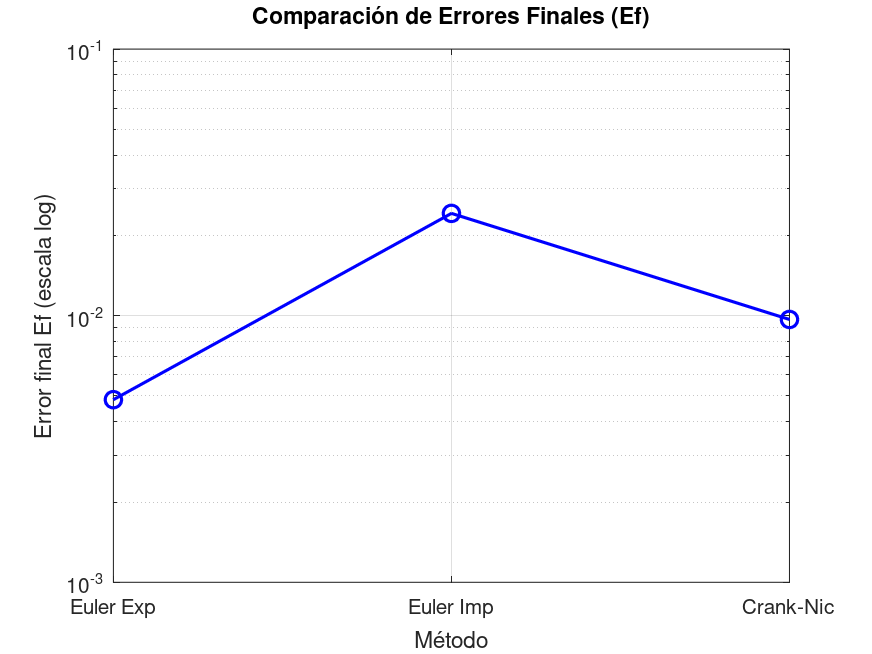
\includegraphics[width=0.6\textwidth]{graficas/grafica_errores.png}
\caption{Comparación de los errores finales \(E_f\).}
\label{fig:errores}
\end{figure}

\begin{figure}[H]
\centering
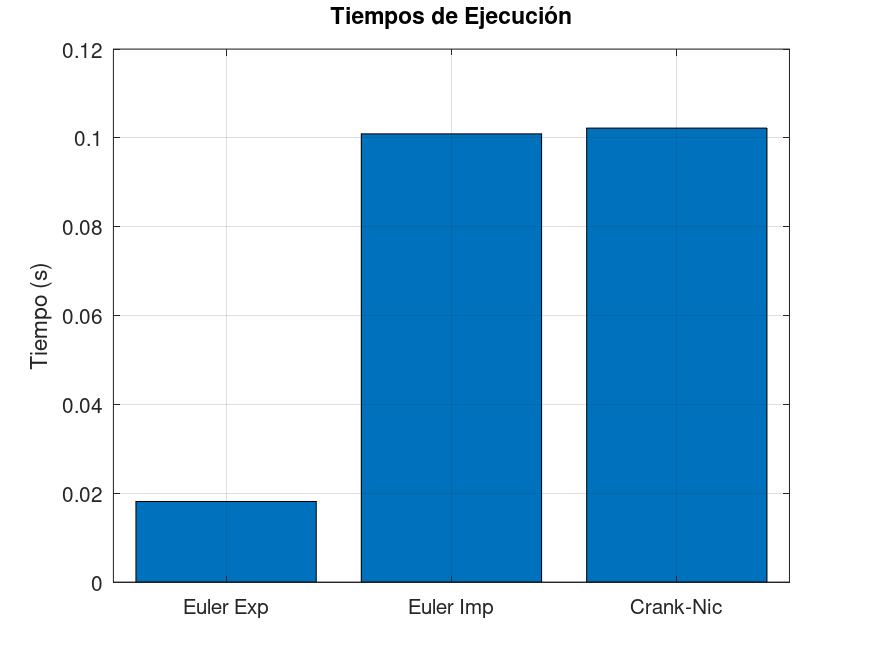
\includegraphics[width=0.6\textwidth]{graficas/grafica_tiempos.png}
\caption{Comparación de los tiempos de ejecución.}
\label{fig:tiempos}
\end{figure}

Los perfiles de temperatura para \(t=0,1,5,10\) s se muestran en las Figuras~\ref{fig:p0} a~\ref{fig:p10}.

\begin{figure}[H]
\centering
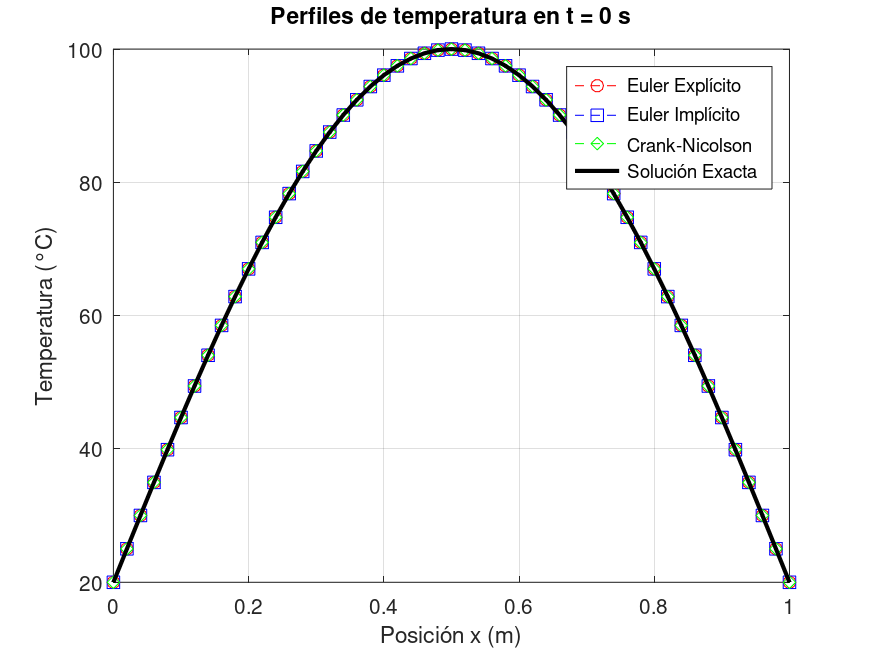
\includegraphics[width=0.6\textwidth]{graficas/perfil_t_0.png}
\caption{Perfiles de temperatura en \(t=0\) s.}
\label{fig:p0}
\end{figure}

\begin{figure}[H]
\centering
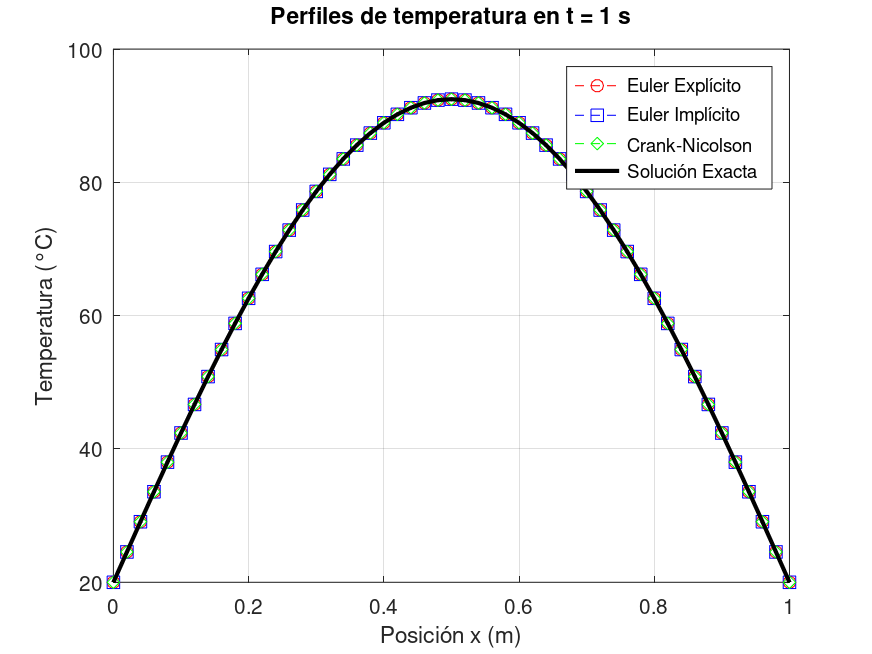
\includegraphics[width=0.6\textwidth]{graficas/perfil_t_1.png}
\caption{Perfiles de temperatura en \(t=1\) s.}
\label{fig:p1}
\end{figure}

\begin{figure}[H]
\centering
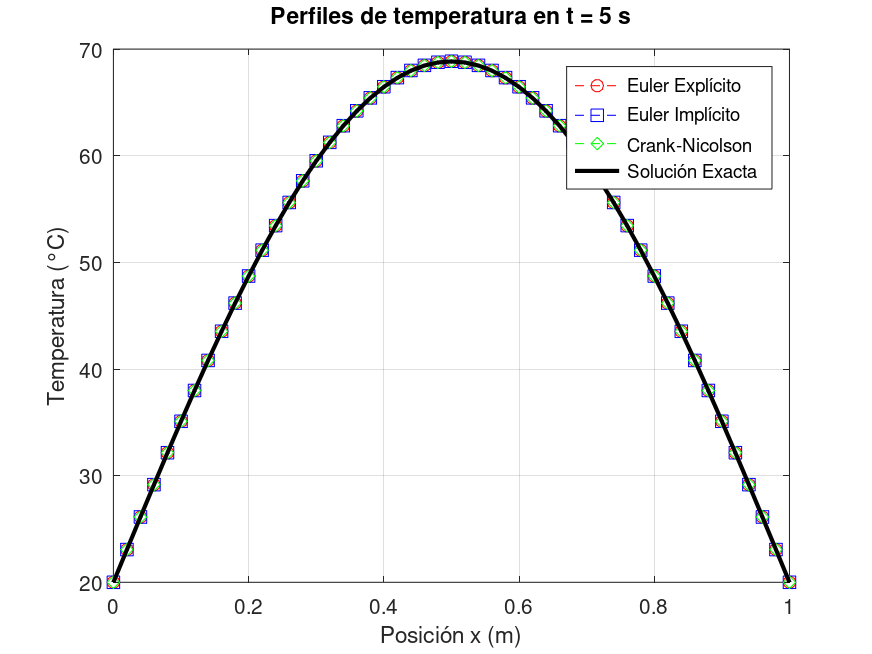
\includegraphics[width=0.6\textwidth]{graficas/perfil_t_5.png}
\caption{Perfiles de temperatura en \(t=5\) s.}
\label{fig:p5}
\end{figure}

\begin{figure}[H]
\centering
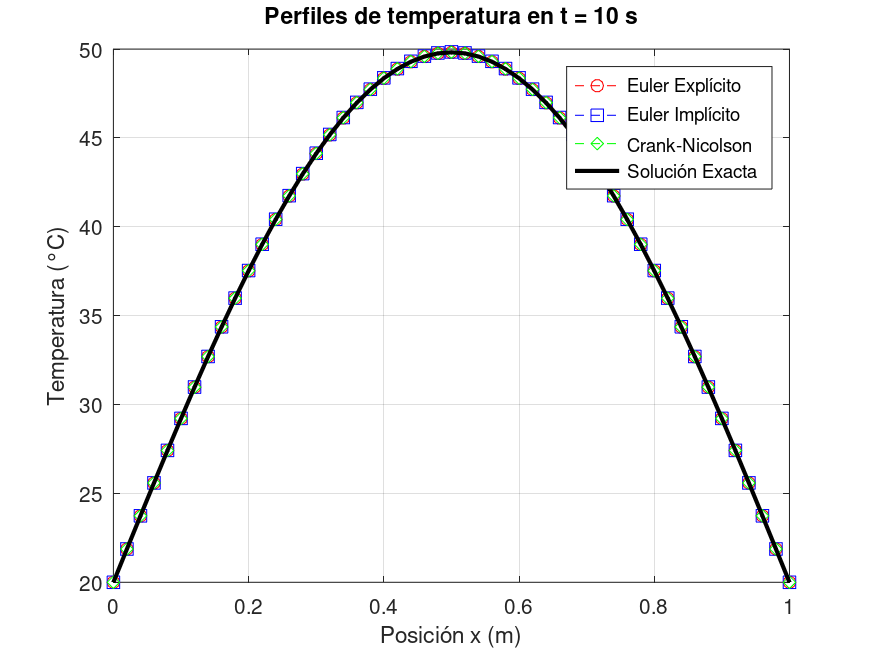
\includegraphics[width=0.6\textwidth]{graficas/perfil_t_10.png}
\caption{Perfiles de temperatura en \(t=10\) s.}
\label{fig:p10}
\end{figure}

% =================================================
\section{Refinamiento de malla}
% =================================================

Se estudió el efecto del refinamiento espacial y temporal con los tres esquemas, manteniendo \(t_f=10\) s. Los resultados se muestran en las Tablas~\ref{tab:espacial} y~\ref{tab:temporal}.

\begin{table}[H]
\centering
\caption{Refinamiento espacial con \(\Delta t = 0.0025\) s.}
\label{tab:espacial}
\begin{tabular}{lcccccc}
\toprule
Método & \(M\) & \(\Delta x\) & \(\Delta t\) & \(\mu\) & \(E_f\) & Tiempo (s) \\
\midrule
Euler exp. & 25 & 0.04000 & 0.0025 & 0.0156 & \(3.503\times10^{-2}\) & 0.061 \\
Euler imp. & 25 & 0.04000 & 0.0025 & 0.0156 & \(4.227\times10^{-2}\) & 0.388 \\
Crank--Nic. & 25 & 0.04000 & 0.0025 & 0.0156 & \(3.865\times10^{-2}\) & 0.400 \\
Euler exp. & 50 & 0.02000 & 0.0025 & 0.0625 & \(6.052\times10^{-3}\) & 0.067 \\
Euler imp. & 50 & 0.02000 & 0.0025 & 0.0625 & \(1.331\times10^{-2}\) & 0.392 \\
Crank--Nic. & 50 & 0.02000 & 0.0025 & 0.0625 & \(9.682\times10^{-3}\) & 0.401 \\
Euler exp. & 100 & 0.01000 & 0.0025 & 0.2500 & \(1.210\times10^{-3}\) & 0.068 \\
Euler imp. & 100 & 0.01000 & 0.0025 & 0.2500 & \(6.050\times10^{-3}\) & 0.448 \\
Crank--Nic. & 100 & 0.01000 & 0.0025 & 0.2500 & \(2.420\times10^{-3}\) & 0.443 \\
\bottomrule
\end{tabular}
\end{table}

\begin{table}[H]
\centering
\caption{Refinamiento temporal con \(M=50\).}
\label{tab:temporal}
\begin{tabular}{lcccccc}
\toprule
Método & \(M\) & \(\Delta x\) & \(\Delta t\) & \(\mu\) & \(E_f\) & Tiempo (s) \\
\midrule
Euler exp. & 50 & 0.02000 & 0.0160 & 0.4000 & \(1.356\times10^{-2}\) & 0.011 \\
Euler imp. & 50 & 0.02000 & 0.0160 & 0.4000 & \(3.289\times10^{-2}\) & 0.067 \\
Crank--Nic. & 50 & 0.02000 & 0.0160 & 0.4000 & \(9.676\times10^{-3}\) & 0.066 \\
Euler exp. & 50 & 0.02000 & 0.0080 & 0.2000 & \(1.936\times10^{-3}\) & 0.021 \\
Euler imp. & 50 & 0.02000 & 0.0080 & 0.2000 & \(2.129\times10^{-2}\) & 0.128 \\
Crank--Nic. & 50 & 0.02000 & 0.0080 & 0.2000 & \(9.680\times10^{-3}\) & 0.131 \\
Euler exp. & 50 & 0.02000 & 0.0040 & 0.1000 & \(3.874\times10^{-3}\) & 0.041 \\
Euler imp. & 50 & 0.02000 & 0.0040 & 0.1000 & \(1.549\times10^{-2}\) & 0.252 \\
Crank--Nic. & 50 & 0.02000 & 0.0040 & 0.1000 & \(9.681\times10^{-3}\) & 0.259 \\
\bottomrule
\end{tabular}
\end{table}

Al refinar la malla espacial, el error disminuye en los tres esquemas. Sin embargo, al refinar únicamente el paso temporal, el error de Euler explícito deja de bajar e incluso aumenta ligeramente cuando \(\Delta t=0.004\) s. Esto ocurre porque el error espacial, que permanece fijo al no cambiar \(M\), comienza a dominar sobre el error temporal. Crank--Nicolson, por ser de segundo orden en tiempo, mantiene su error prácticamente constante, lo que confirma que el error espacial es el que predomina. 

Esto es consistente con los órdenes teóricos de los esquemas: Euler explícito e implícito son de orden \(O(\Delta t) + O(\Delta x^2)\), mientras que Crank--Nicolson es de orden \(O(\Delta t^2) + O(\Delta x^2)\). Por ello, al refinar únicamente el paso temporal, el término \(O(\Delta x^2)\) se vuelve el error dominante y el error total deja de disminuir.

% =================================================
\section{Estabilidad de Euler explícito}
% =================================================

Para estudiar la estabilidad se utilizó \(M=50\) y dos valores de \(\mu\): 0.4 y 0.6, con una perturbación interior de \(10^{-6}(-1)^i\) que se anula en los extremos. Los resultados se muestran en las Figuras~\ref{fig:est04} y~\ref{fig:est06}.

\begin{figure}[H]
\centering
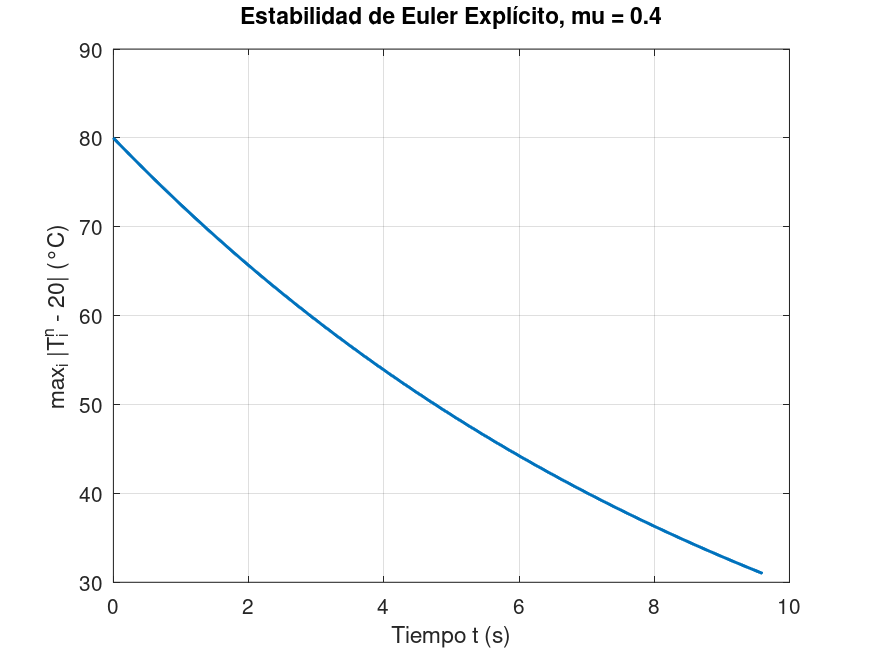
\includegraphics[width=0.6\textwidth]{graficas/estabilidad_mu_0.4.png}
\caption{Estabilidad de Euler explícito con \(\mu=0.4\).}
\label{fig:est04}
\end{figure}

\begin{figure}[H]
\centering
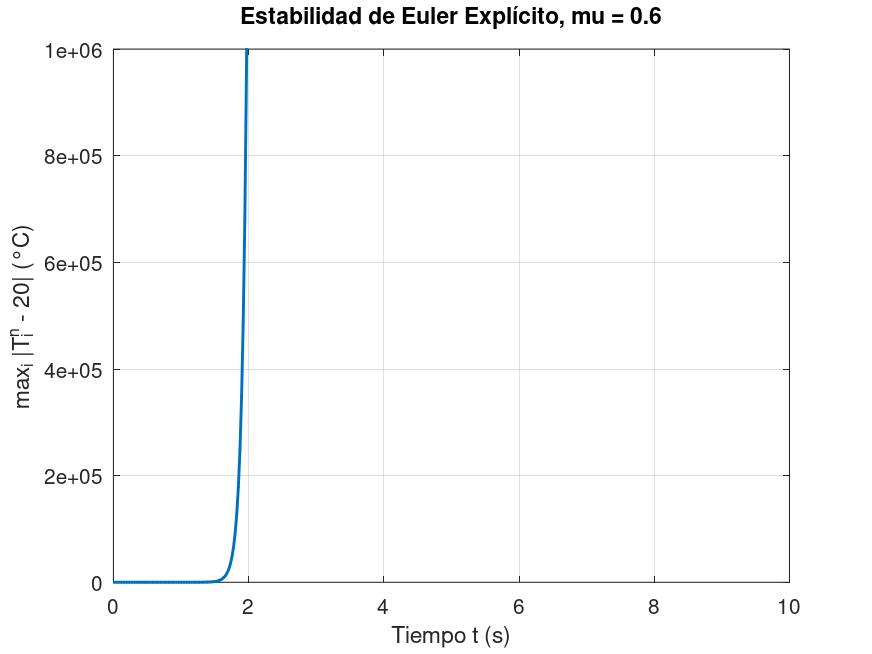
\includegraphics[width=0.6\textwidth]{graficas/estabilidad_mu_0.6.png}
\caption{Estabilidad de Euler explícito con \(\mu=0.6\).}
\label{fig:est06}
\end{figure}

Con \(\mu=0.4\) la desviación máxima se mantiene en 80, lo que indica que el esquema es estable. Con \(\mu=0.6\) la solución crece sin control y supera \(10^6^\circ\)C en \(t=1.992\) s, confirmando la inestabilidad teórica del esquema cuando \(\mu>0.5\).

% =================================================
\section{Tiempo de enfriamiento}
% =================================================

Se utilizó Euler implícito con \(M=50\), \(\Delta t=0.01\) s y \(t_f=30\) s. El primer tiempo de la malla en que la temperatura máxima es menor o igual a \(30^\circ\)C resultó \(t=21.09\) s, con una temperatura máxima en el paso anterior de \(30.0064^\circ\)C. El tiempo analítico exacto es \(t=21.069\) s, por lo que la diferencia es de apenas \(0.0208\) s, atribuible al redondeo al siguiente paso de la malla temporal.

% =================================================
\section{Mapa de calor y temperatura en el centro}
% =================================================

En la Figura~\ref{fig:mapa} se muestra el mapa de calor de \(T(x,t)\), y en la Figura~\ref{fig:centro} la temperatura en el centro de la barra junto con el umbral de \(30^\circ\)C.

\begin{figure}[H]
\centering
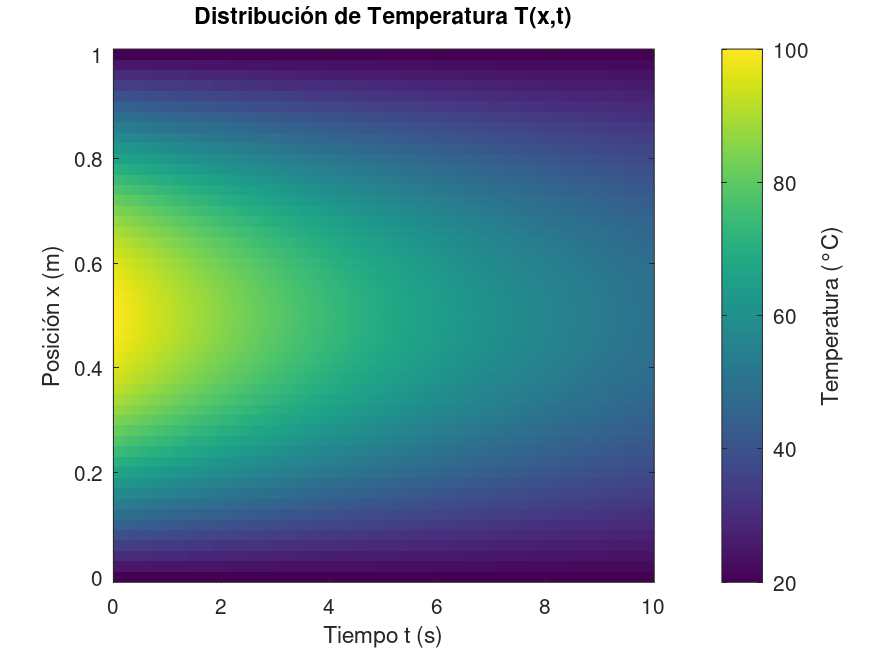
\includegraphics[width=0.7\textwidth]{graficas/mapa_calor.png}
\caption{Mapa de calor de la distribución de temperatura \(T(x,t)\).}
\label{fig:mapa}
\end{figure}

\begin{figure}[H]
\centering
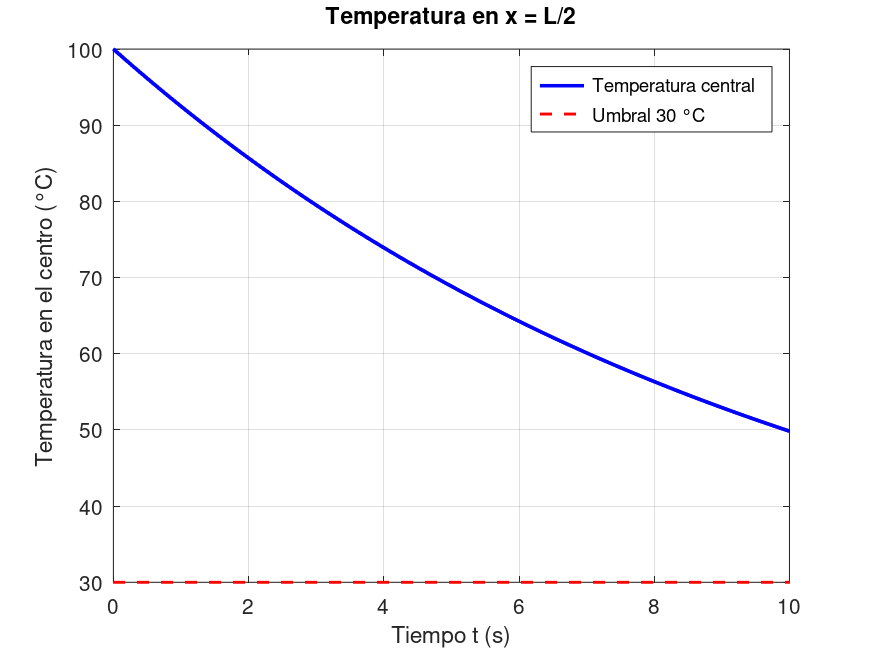
\includegraphics[width=0.6\textwidth]{graficas/temperatura_centro.png}
\caption{Temperatura en el centro de la barra y umbral de \(30^\circ\)C.}
\label{fig:centro}
\end{figure}

% =================================================
\section{Análisis de resultados}
% =================================================

Los resultados muestran que los tres esquemas aproximan correctamente la solución, aunque con diferencias en precisión y costo. Euler explícito es el más rápido porque no resuelve sistemas lineales, pero está condicionado por la restricción \(\mu \le 0.5\). Euler implícito y Crank--Nicolson son estables para cualquier \(\mu\), aunque requieren resolver un sistema en cada paso temporal. En este caso, el Gradiente Conjugado convergió en una sola iteración por paso, lo que explica que los tiempos de ambos esquemas sean similares.

En cuanto a la precisión, Crank--Nicolson presenta un error menor que Euler implícito, lo cual es consistente con su orden dos en tiempo. Euler explícito, en el régimen estable, también ofrece errores bajos, pero su dependencia de la condición de estabilidad limita su uso con pasos temporales grandes.

El refinamiento de la malla mostró que el error total depende tanto del paso espacial como del temporal. Refinar solo una de las dos variables puede dejar de reducir el error cuando la otra contribución domina, como se observó en el refinamiento temporal de Euler explícito.

Finalmente, el tiempo de enfriamiento numérico coincidió con el analítico dentro de un paso de la malla temporal, lo que valida la implementación. El mapa de calor y la temperatura en el centro confirman que la barra se enfría de manera uniforme hacia los \(20^\circ\)C impuestos en los extremos, con la temperatura máxima inicial en el centro que disminuye con el tiempo.

% =================================================
\end{document}